\documentclass[11pt]{article}
\usepackage{amsmath}
\usepackage{algpseudocode,algorithm}
\usepackage{algpseudocode}
\usepackage{tikz}
\usetikzlibrary{trees}
\setlength{\topmargin}{-0.7in}

\setlength{\textwidth}{6.5in}

\setlength{\oddsidemargin}{0.0in}

\setlength{\textheight}{10.0in}

\setlength{\parindent}{0in}

%\renewcommand\arraystretch{0.0}
\renewcommand\arraystretch{2.4}
%\setlength\minrowclearance{2.4pt}

\renewcommand{\baselinestretch}{1.2}
\newcommand{\problem}[1]{ \medskip \pp $\underline{\rm Problem\ #1}$\\ }
\newcommand{\ans}{\textbf{Answer: }}
%\newlength{\pagewidth}
%\setlength{\pagewidth}{6.5in}
\pagestyle{empty}

%\def \A{\rm At}
\def\pp{\par\noindent}

\begin{document}

\begin{flushleft}
CSOR W4231.002 -- Spring, 2016
\end{flushleft}

%\begin{flushright}
%Eleni Drinea
%\end{flushright}

%\vspace{0.5in}
 \centerline{\bf Homework 1}
\medskip
\centerline{Shivam Choudhary (sc3973)}
\centerline{Due: 8pm, Monday, February 8, 2015}

\medskip 

\bigskip



\begin{enumerate}

\item(25 points) In the table below, indicate the relationship between functions $f$ and $g$ 
for each pair $(f, g)$  by writing  ``yes" or ``no"  in each box. For example, 
if $f=O(g)$ then write ``yes"  in the first box. Here $\log^b{x} = (\log_2{x})^b$.


\begin{table}[tbh] \begin{center}
\begin{tabular}{|c|c|c|c|c|c|c|}\hline  % \label{tab: less}
$f$ & $g$ & \ \ $O$ \ \  & \ \  $o$ \ \   &  \ \ $\Omega$ \ \  &  \ \ $\omega$ \ \ & \ \ $\Theta$  \ \ \\ \hline
$\log^2{n}$ & $25\log{n}$  &no  &no  &yes    & yes & no \\ \hline
$\sqrt{ \log{n} }$ & $(\log{ \log{n}})^4$  & no  &no  &yes    &  yes&no \\ \hline
$3n \log{n}$ & $n\log{3n}$  &  yes &no  &yes    &no  &yes \\ \hline
$n^{3/5}$ & $\sqr{n}\log{n}$  & no  &no  &  yes   &yes  &no \\ \hline
$\sqrt{n} + \log{n}$ & $2\sqrt{n}$  & yes  &no   &   yes    & no&    yes \\ \hline
$n^2 2^n$ & $3^n$  &yes  &yes  &  no  &no  &no \\ \hline
$\sqrt{n} 2^n$ & $2^{n/2+\log{n}}$  &no &no  &yes    &yes  &no \\ \hline
$n \log{3n}$ & $\frac{n^2}{\log{n} }$  &  yes &yes  &no    &no  &no \\ \hline
$n!$ & $2^n$  &no  &no &yes    &yes  &no \\ \hline
$\log{n!}$ & $\log{n^n}$  & yes  &no  & yes   &no  &yes \\ \hline
\end{tabular}
\end{center}
\end{table} 

\newpage
%\item 
%(a) (4 points) Find (with proof) a function $f_1$ such that $f_1(2n)$  is $O(f_1(n))$. 
%(b) (4 points) Find (with proof) a function $f_2$ such that $f_2(2n)$  is not $O(f_2(n))$.


\item (12 points)
Show that, if $\lambda$ is a positive real number, then $f(n)= 1+ \lambda + \lambda^2 + \ldots + \lambda^n$ is
\begin{enumerate}  
\item $\Theta(1)$ if $\lambda<1$. 
\item $\Theta(n)$ if $\lambda=1$.
\item $\Theta(\lambda^n)$ if $\lambda>1$.
\end{enumerate}
\ans
\begin{center}
f(n) = $\frac{1 - \lambda^{n+1}}{1-\lambda }$ = $\frac{ \lambda^{n+1}-1 }{\lambda -1 }$ respectively as $\lambda >1$ or $\lambda <1$,when $\lambda$ $\neq 1$ 
\end{center}
(a) According to the definition of $\Theta{(g(1))} $, the bounds are defined as c1 $\leq$ f(n) $\leq$ c2.Since 1-$\lambda^{n+1}$ will always be less than 1-$\lambda$,we can always find two constants c1($\leq 0,0.5$) and c2($\geq1,1.5$). Hence the sum f(n) is bounded by $\Theta(1).$

(b) $\Theta(n)$ if $\lambda=1$. For $\lambda=1$ 
f(n)=n+1 for this case. So $\Theta{(n)} \implies$
c1 n $\leq$ n+1 $\leq$ c2 n.
And this translates to c1 being any quantity $\leq$ 1 and c2 being any quantity $\geq$ 1.Since we can find c1 and c2,$f(n)$ is bounded by $\Theta(1)$

(c) As $\lambda \geq1 $ so, $\lambda^n \geq 1$. For lower bound we can use the relation $\lambda^{n+1}-\lambda^{n}\leq \lambda^{n+1}-1$.

Now dividing both sides by $\lambda -1 $, it becomes 
\begin{center}
$\lambda^n\leq f(n)$,which is lower bound $\Omega(\lambda^n)$
\end{center}
For the upper bound let us consider the inequality $\lambda^{n+1}-1 \leq \lambda^{n+1}$. Again dividing both sides of the inequality by $\lambda -1$ we get 
\begin{center}
$f(n) \leq \frac{\lambda^{n+1}-1}{\lambda}$\\
Quickly the right side of the inequality can be simplified to $(\lambda^n)* \frac{\lambda}{\lambda -1 } $
\end{center}
This gives us our upper limit $O(\lambda ^n)$. Combining the bounds $\Omega(\lambda^n)$ and $O(\lambda^n)$ we get the bounds to be $\Theta{(\lambda^n)}$

\bigskip

\item (12 points)
\begin{itemize}
\item Find (with proof) a function $f_1$ such that $f_1(2n)$  is $O(f_1(n))$. 

\ans Let $f_1(n)$ = $\frac{n}{2}$, Now $f_1(2n)$ = n and $O(f_1(n))$ = n. Hence proved. So for all linear functions of the form AX+B it will hold true.
\item Find (with proof) a function $f_2$ such that $f_2(2n)$  is not $O(f_2(n))$.

\ans Let $f_2(n)$ = $2^n$ so $O(f_2(n))$ = $2^n$. Now $f_2(2n)$ = $2^{2n}$ which is $O(4^n)$ and hence $f_2(2n)$ $\neq$ $O(f_2(n))$. This infact would be true for all exponential functions.
\item Give a proof or a counterexample: if $f$ is $o(g)$ then $f$ is $O(g)$.

\ans Borrowing from Question 1, $f(n)$ = $n^2 2^n$ and $g(n)$ = $3^n$. In this case we can see that $f(n)$ is both $O$ and $o$ for $g(n)$. Hence this serves as a counterexample that they both can be equal.

\end{itemize}

\bigskip

\item (24 points) Consider an array $A$ consisting of $n$ integers, $A[1], A[2], \ldots, A[n]$.
You want to output a two-dimensional $n$-by-$n$ array $B$ such that for all
$i<j$, $B[i, j]$ contains the sum of array entries $A[i]$ through $A[j]$, that is,
$A[i]+ A[i+1] + \ldots + A[j]$. (For $i \geq j$, the value of entry $B[i,j]$
is left unspecified, so we don't care what is output for these values.)

The most natural way to solve this problem is provided by the following algorithm. 
\begin{algorithmic}
\State \For{ $i=1, 2, \ldots, n$}
 \For{ $j=i+1, i+2, \ldots, n$}
\State Add up array entries $A[i]$ through $A[j]$
\State Store the result in $B[i,j]$
\EndFor
\EndFor
\end{algorithmic}

\begin{enumerate}


\item (6 points) Let $T(n)$ denote the running time of this algorithm  on an input of size $n$. 
For a function $f$ of your choice, show that $T(n)$ is  $O(f(n))$\\
\begin{algorithm}\begin{center}
\caption{Array Adder }\label{euclid}
\begin{algorithmic}[1]
\For{i=0; i$\textless$ARRAYSIZE; i++}
\For{j=i+1; j$\textless$ARRAYSIZE; j++}
\State sum=0
\For {k=i; k$\leq$j; k++}
\State sum+=A[k]
\EndFor
\State b[i][j]=sum
\EndFor
\EndFor
\end{algorithmic}
\end {center}
\end{algorithm}

\ans
Let f(n) be the combined complexity of all the three for loops. Now since the algorithm does not depend on best/worst case scenario, we can see that Line 1 has complexity of $O(n)$ and similarly for Line 2 and Line 4. This means that the total complexity of the algorithm is $O(n^3)$. In other words the algorithm cannot be made to give better performance in some cases(dependent on type of input.)


\item (6 points) For the same function $f$, show that $T(n)$ is also $\Omega( f(n) )$. 

\ans All the three loops run independently i.e their is no best case/worst case. Therefore just being dependent on array size all the loops would run $\Omega(f(n))$ = n for each loop and since we have three loops  it will be $\Omega(n^3)$. And since there is no best/worst case this serves as a tight bound for the function. 

This also gives us the idea that this implementation is $\Theta(n^3)$
\newpage

\item (12 points) Give a different algorithm for this problem with running time $T'(n)$ 
that is asymptotically better than $T(n)$. In other words, you should show 
that the running time of your new algorithm satisfies $T'(n)= O(g(n))$ for
some function $g(n) = o( f(n) )$.  \\
{\em Hint: The new algorithm should exploit 
the structure of the problem better.}

The same can be achieved by using two for loops as shown in the below pseudocode.

\begin{algorithm}
\caption{Array Adder Modified}\label{euclid}
\begin{algorithmic}[1]
\For{i=0; i$\textless$ARRAYSIZE; i++}
\State last=A[i]
\For{j=i+1; j$\textless$ARRAYSIZE; j++}
\State last+=a[j]
\State b[i][j]=last
\EndFor
\EndFor
\end{algorithmic}
\end{algorithm}
Again let Line 1 runs N times and has complexity of $O(n)$. Now since we have two for loops and no other condition to distinguish between cases(like worst/best) the algorithm will run in time $O(n^2)$ in all the cases which means that the algorithm would be again $\Theta(n^2)$. This does offer improvement over the previous algorithm which had running time of $O(n^3)$

\end{enumerate}


\item (16 points) Give tight asymptotic bounds for the following recurrences.
\begin{itemize}
\item $T(n) = 4T(n/2)  + n^3 -1$.
\ans $O(n^3)$
\item $T(n) = 8T(n/2) + n^2$.
\ans $O(n^3)$
\item $T(n) = 6T(n/3) + n$.
\ans $O(n^{log_3 6})$
\item  $T(n) = T(\sqrt{n})  + 1$.
\ans $O(loglogn)$
\end{itemize}

\bigskip


\item (31 points) The Fibonacci numbers are defined by the recurrence 
\begin{eqnarray}
&& F_0 =  0, F_1=1 \nonumber \\
&& F_n =  F_{n-1} + F_{n-2}  (n \geq 2) \nonumber 
\end{eqnarray}
\begin{enumerate}
\item (4 points) Show that $F_n \geq 2^{n/2}$, $n \geq 6$. 

\ans Proof By Strong Induction
\begin{table}[tbh]  
\begin{center}
\begin{tabular}{|c|c|c|c|c|c|c|c|c|}\hline  % \label{tab: less}
$n$ & $0$ \ \ & $1$& $2$& $3$& $4$& $5$& $6$& $7$\\ \hline
$F_n$ & $0$ & \ \ $1$ \ \  & \ \  $1$ \ \   &  \ \ $2$ \ \  &  \ \ $3$ \ \ & \ \ $5$  \ \ &\ \ $8$ \ \ &\ \ $13$\\ \hline
\end{tabular}
\end{center}
\end{table} 
\newpage
Since it is required to prove to n$\geq$ 6, without loss of generality we can assume this to be the base case.
$F_6$ = 8 and $2^3$ = 8 which shows that base case is true.\\
Now Let the condition be true for some n and also for values below that n.
Then we can write 

$F_n \geq 2^\frac{n}{2}$  and for n+1 the condition $F_{n+1} \geq 2^\frac{n+1}{2}$ has to be proven to be true.

So using the recurrence definition the proof reduces down to :-
$F_n + F_{n-1} \geq 2^\frac{n+1}{2}$

Now since our assumption says that the term $F_n$ are atleast $2^\frac{n}{2}$ and correspondingly we get $2^\frac{n}{2}+ 2^\frac{n-1}{2} \geq 2^\frac{n+1}{2}$ which is true as it reduces down to $1.7*2^\frac{n}{2}$ and $1.414*2^\frac{n}{2}$.




Hence our assumption is true and the equation holds for all $n\geq 6$.
\item  Assume that the cost of adding, subtracting, or multiplying two integers is $O(1)$, independent 
of the size of the integers.
\begin{itemize}
\item (4 points) Write pseudocode for an algorithm that computes $F_n$ based on the recursive definition above. 
Develop a recurrence for the running time of your algorithm and 
give an asymptotic lower bound for it.

\ans 
\begin{algorithm}
\caption{Recursive Fibonacci}\label{euclid}
\begin{algorithmic}[1]
\Procedure{fib}{n}
\State if $n==1$
\State return 1
\State if $n==0$
\State return 0 
\State Else 
\State return fib(n-1)+fib(n-2)
\EndProcedure
\end{algorithmic}
\end{algorithm}

For $\Omega(f(n))$ to exist we should be able to find a constant c such that its always greater than $f_n \geq$c*f(n). We observe one property of this series as $f(n)\geq f(n-1)$ and it can be generalized as 
$f(n) = f(n-1)+f(n-2) + c$ so $f(n)\geq 2*f(n-2)+c$ which can be further generalized as $f(n)\geq 2^kf(n-2k)+c$. I chose to omit series which occurs in c as its highest power is $2^{k-1}$ and the first term has leading power to be $2^k$. Now the series terminates at n=2k or k=n/2,which gives f(0). Hence plugging back the power we get $f(n)\geq 2^\frac{n}{2}$. Hence the $\Omega(2^\frac{n}{2})$ is the lower bound for this recurrence.
\item (4 points) Write pseudocode for a non-recursive algorithm that asymptotically performs fewer
additions than the recursive algorithm. Discuss the running time of the new algorithm.

\ans 
\begin{algorithm}
\caption{Iterative Fibonacci}\label{euclid}
\begin{algorithmic}[1]
\Procedure{ifib}{n}
\For{i=0;i<n-2;i++}
\State first = second
\State second = third
\State third = first+second
\EndFor
\State third
\EndProcedure
\end{algorithmic}
\end{algorithm}
The running time of this algorithm is $O(n)$. Also since this algorithm does not have any other cases to check upon it's lower bound is $\Omega(n)$. Also this translates to $\Theta(n)$ which are the bounds for this algorithm.
\newpage
\item (10 points) Show how to compute $F_n$ in $O(\log{n})$ time 
using only integer additions and multiplications. \\
{\em (Hint: Express $F_n$ in matrix notation
and consider the matrix $${0 \ \ \ 1} \choose {1\ \ \  1} $$
 and its powers.)}
%Provide an upper bound for the running time of this algorithm.

\ans  Expressing the matrix in the form as given below. We can see that $F_n$ = $Matrix^n-1$
\begin{center}
\begin{bmatrix}
    $F_{n+1}$       & $F_{n}$ \\
    $F_{n}$       & $F_{n-1}$ \\
\end{bmatrix}
\end {center}
So calculating the recurrence for the computation by drawing the recurrence tree.


\end{itemize}

\begin{center}
\begin{tikzpicture}[level distance=1.5cm,
level 1/.style={sibling distance=3.5cm},
level 2/.style={sibling distance=1cm}]
\tikzstyle{every node}=[circle,draw]
    \node (Root)  {$M^n$}
        child  {
        node {$M^\frac{n}{2}$}
        child { node {$M^\frac{n}{4}$} }
        child {node{$M^\frac{n}{4}$}}
    }
    child  {
        node {$M^\frac{n}{2}$}
        child { node {$M^\frac{n}{4}$} }
        child {node{$M^\frac{n}{4}$}}
    };

\end{tikzpicture}
\end {center}
And so on, the tree goes till 1 and the depth of the tree is $log n$($n/2^i$,$i=logn$). Now since the multiplication will yield the matrix M and there are $log n$ such operations and multiplication requires $O(1)$ time so the full operation takes $O(logn)$.
\item (9 points) Now assume that adding two $m$-bit integers requires $\Theta(m)$ time 
two $m$-bit integers requires $\Theta( m^2 )$ time. What is the running time of the three
algorithms under this more reasonable cost measure for the elementary arithmetic operations?
\newpage

\ans We can assume that $m$ = $logn$ for representing the numbers.
\begin{enumerate}
    \item For recursive since we add two values on each step, so from the previous discussion in the same problem now we just need to add $logn$ more. Now this means the equation changes to $2^n*logn$ which gives the asymtotic upper bound. For the asymtotic lower bound it becomes $2^{n/2}*logn$
    \item For Iterative process it is straight forward,  each addition steps now takes log n time and we have n such steps,hence the complexity becomes n*logn.
    \item For the Matrix process since now each multiplication takes $log^2n$ time and we have $log n$ such combinations,so the total complexity is $O(logn*log^2n)$ which is $O(log^3n)$
\end{enumerate}

\end{enumerate}




\end{document}

